\documentclass[10pt,a4paper]{book}
\usepackage[utf8]{inputenc}
\usepackage[T1]{fontenc}
\usepackage{amsmath}
\usepackage{amsfonts}
\usepackage{amssymb}
\usepackage{graphicx}
\usepackage[cache=false]{minted}
\usemintedstyle{colorful}
%\definecolor{bg}{HTML}{282828} % from https://github.com/kevinsawicki/monokai
%\setminted{bgcolor=bg,breaklines=true}
\setminted{breaklines=true}
\begin{document}
\title{Data Structures}
\author{Andrew Rosen}
\date{}
\maketitle
\tableofcontents




\chapter{Introduction}

\section{What is a Data Structures Course}
Data Structures is all about defining the different ways we can organize data.


\section{Why This Book?}

\subsection{Where Does This Book Fit Into a Computer Science Curriculum }

Education in Computer Science is based around three core topics: translating the steps of solving a problem into a language a computer can understand, organizing data for solving problems, and techniques that can be used to solve problems. % reword
These courses typically covered in a university's introductory course, data structures course, and algorithms course respectively, although different universities decide exactly what content fits in which course.
Of course, there is are lot more concepts in computer science, from operating systems and low level programming,  to networks and how computers talk to each other. However, all these concepts rely on the knowledge gained in the core courses of programming, data structures, and algorithms.

 

This textbook is all about Data Structures, the middle section between learning how to program and the more advanced problem solving concepts we learn in Computer Science. 
Here, we focus on mastering the different ways to organize data, recognize the internal and performative differences between each structure, and learn to recognize the best (if there is one) for a given situation.


\subsection{What Are My Base Assumptions about the Reader?}

This textbook assumes that the student has taken a programming course that has covered the basics.
Namely: data types such as ints, doubles, booleans, and strings; if statements, for and while loops; and object orient programming.
The first writeup of the textbook will be done in Java, but I will try to add as much Python into the book as well.


\section{To The Instructor}


\section{To The Student}


%\section{Science and Art}


\chapter{The Array}

\section{Array Operations}

\section{Finding Values in an Array}

\chapter{Analyzing Algorithms}

\subsection{Cost}
Every function, operation, algorithm, or what have you that a computer performs has a \emph{cost}. In fact, there are always multiples costs;  we often just focus on the most important one or two costs.  
What is most important depends on context.

However, when we measure cost, we need to do abstractly.  
When we measure the amount of time that an algorithm takes

\subsubsection{Time}
A time cost is a measure of not just how long it takes a program to finish executing, bit also how the length of execution is affected by adding additional item.

Time is almost always \emph{the most important cost}.

\subsubsection{Space}
\subsubsection{Energy}
\subsubsection{Other costs - Bandwidth}

\section{Big O Notation}
\subsection{Space Complexity}

\section{The Formal Mathematics of Big O Notation}
\section{Other Notations}

\chapter{Array Lists}
The first data structure we will be studying is the list.
The list is by far the most relatable data structure, as humans deal with lists on a regular basis.

\section{What is a list?}
When you get right down to it, lists are defined by order.


\begin{minted}{Java}
public static <E> boolean isPermutation(List<E> listA, List<E> listB) {
	
	if(listA.size() != listB.size()) {
		return false;
	}
	for(int i  = 0; i < listA.size() ; i++){
		E item =  listA.get(i);
		int countA = 0;
		int countB = 0;
		
		for (E element : listA) {
			if(item.equals(element)){
				countA++;
			}
		}
		for (E element : listB) {
			if(item.equals(element)){
				countB++;
			}
		}
		if(countA != countB) {
			return false;
		}
	}
	return true;
}
\end{minted}



\section{ArrayLists}
An array list, as you might have guessed, are lists built using \textit{arrays}.\footnote{Shockingly, many of the names we give things at this point actually make sense.}
They work by growing or shrinking the array\footnote{A lie.  As you'll see we don't actually change the size of an array;  we create a new array of the appropriate size and copy everything over} automatically as items are added or removed from the list, giving the illusion that the data structure can hold an arbitrary amount of data.

We'll go into the specifics of how this works in Section \ref{buildingArraylist}.


\subsubsection{Python's Lists}
Python's lists, such as below:
\begin{minted}{python3}
l = [1,2,3] # this is a list, not an array!	
\end{minted}
are actually array lists! %TODO cite this https://docs.python.org/3/faq/design.html#how-are-lists-implemented-in-cpython

Python uses a different vocabulary for some of the methods we'll be implementing below.  
For example, take the action of adding an item to a list.
Python uses the \texttt{append} method to add an item to end of the list and \texttt{insert} to put an item into the middle of the list.
Java (who's vocabulary we'll be following), uses \texttt{add} for both these contexts. 



\section{Generics}
\section{Building an ArrayList}
\label{buildingArraylist}

\subsection{More Restrictive or Permissive Generics}

\section{Analysis}
\chapter{Linked Lists}
Linked lists , also referred to as reference based lists , are the second type of lists typically seen in applications . To be clear a linked list is a list. That means it could be used anywhere an array list can.   So Why do we have two objects that are functionally equivalent , two collections that hold things in order, using indexes?  The answer is will see, is because each list is good at the thing the other list is less efficient at.


Array based lists use contiguous blocks of memory, allocated all at once and when then capacity of the list is filled up.  Utilizing an array makes these types of lists extremely efficient at retrieving an item from a specific index, but adding items anywhere but the end of the list incurs a $O(n)$ runtime.



Linked Lists can do all the things an Array List can, but the underlying structure is completely different.  
Each item in the list is stored in an Object called a \textit{Node}.  Nodes are created as items are added to list, rather than in advance.  This means that are not contiguous, but Rather they are scattered throughout the computer's memory . So how in the world do we keep track of where we've stored all these items ? The solution resembles the scavenger hunt through the computer's memory.  Each node Not only the memory location of the item that is being stored, but the memory location of the next node in the list . An example of this code can be found below\footnote{Why is this class private in Java \texttt{private}? An inner class  (or private class) is a class that lives within another class.  We use this for two reasons:  Our nodes only exist to build the linked list, so they don't need to have their own class.  The Second reason is   What about \texttt{static class}? This means that we can create nodes without having to make a Linked List first! }: %TODO Check this.

\begin{minted}{Java}
// a snippet of the Node Class
// This will live inside the LinkedList class
private static class Node<E> {
	E item;
	Node<E> next;
	
	public Node(E item) {
		this.item =  item;
	}
} 
\end{minted}
Upon first glance, this code may be very confusing. Each node class contains a reference to a node inside of it.  This may give the impression that nodes  situated one inside another, like one of those Russian nesting matryoshka dolls.  
However, keep in mind what the node is actually storing is not other objects, but instead memory locations of where to find them.
This means that our linked list is more akin to a scavenger hunt where each objective in the hunt contains the instructions on how to find the next objective.

In other words, the item Is the data that is being stored (well actually the memory location, don't forget that ) , and next refers to the memory location of the next index in the list.  Crash course is an excellent video demonstrating this which you can find here: %TODO: Link video


\section{Connecting Nodes into a list.}
%TODO





we keep track of only the first and last item in the list, referred to as the head and the tail . 


I will be presenting the directions to building a fully functional  singly-linked list and doubly-linked list.  
These directions will differ from the mechanics of how your programming language of choice implements them, but have the same time complexity for their operations.
My implementation is constructed with the goal of making the code easy to understand and the decisions that need to be for adding and removing reflect each other.
Finally, my code aims to minimize the number of null-pointer exceptions and their ilk a programmer would make.

The full implementations can be found at the end of the Chapter.

\section{Building a Singly LinkedList}
We open up our linked list with a class declaration. 
If our language uses generics, we specify it there.
I'll be choosing not to inherit from the built-in list so we can focus solely on our own code and no external distractions.


In Java, our code begins like this.
\begin{minted}{Java}
public class LinkedList<E> { }
\end{minted}


In Python
\begin{minted}{python3}
class LinkedList(object):
	pass
\end{minted}


\subsection{The Node}
We want the Node class to be a private/internal class, so that the Node we write for a singly linked list and doubly linked list won't get mixed up in our coding environments.
This also applies for other data structures that will be using nodes.

\begin{minted}{Java}
public class LinkedList<E> { 
	
	private static class Node<E>{
		E item;
		Node<E> next;
		
		public Node(E item){
			this.item = item;
		}
	}
}
\end{minted}

\begin{minted}{python3}
class LinkedList(object):
	class Node(object):
		def __init__(self, item) -> None:
			self.item = item
			self.next = None

	pass
\end{minted}

In the Node private/internal/inner class (and only there), the \texttt{this} or \texttt{self} refers to the \textbf{node} rather than the linked list.





\subsection{Instance Variables and Constructor}

Our linked list Linkedlist only needs a few Instance  variables in order to Function. We need to keep track of the size; Without it we would have no idea what the valid indices are in the list. We need to keep track of the head so we know where to start our scavenger hunt for any particular index or item we're looking for.  Finally we'll keep track of the tail . While keeping track of the tail isn't strictly necessary , keeping track of it means that will be able to add an item to the end of the linked list very efficiently (\texttt{O(1)}).

The only job of the constructor is to initialize everything to either zero or null.

Finally, it's probably a good idea to go ahead and write getter method for the size of the list.

\begin{minted}{Java}
public class LinkedList<E> { 
	private int size;
	private Node<E> head;
	private Node<E> tail;
	
	public int size(){
		return this.size;
	}
}
\end{minted}






\subsection{Adding}
Our Linked list has two add methods, just like the array list.  The first only takes in an item and adds that item to the end of the linked list . It will do this by calling our second method which takes in an index and an item and inserts that item at that index.\footnote{If this sounds familiar, it's because this is precisely what the add method in the arraylist does. Shocking, right?}

Let's take a look at our first add\footnote{As with the arraylist , the add method returns a boolean to signify that we were successfully able to add it to the list . This will always be true, but we do this because Java expects this for collections, as explained in arraylists } method:

\begin{minted}{Java}
public boolean add(E item){
	this.add(this.size, item);
	return true;
}
\end{minted}

\begin{minted}{Python3}
def add(self, item):
	self.add(self.size, item)
	return True
\end{minted}

Simple enough!  But what about that second add method?
When we do any kind of operation on a linked list, we need to think about how instance variables in a linked list will be altered. 
Fortunately, we only have three instance variables: \texttt{size}, \texttt{head}, and \texttt{tail}.
When adding to a linked list, the size will always be altered as long as the index is valid.
Our list's \texttt{head} will only be altered when we add an item to the beginning of the list and our \texttt{tail} will only be altered when we add to the end of the list.  If the list is empty , then the node for that added item becomes both the head and the tail.



We can simplify our job by breaking the add method into five separate cases:
\begin{enumerate}
	\item The index that we want to add to is out of bounds.
	\item We are adding an item to a list that is completely empty. This is going to change the head and tail the list from nolta something. 
	\item We are adding an item to index 0, which is going to change the head of the list.
	\item We are going to add an item to the end of the list, which means that we are going to change what the tail is.
	\item We are adding to some other index in the list , which means that we don't have to bother changing the head or the tail.
\end{enumerate}


Let's start with the first case.

\subsubsection{Checking the index is in or out of bounds}




Since we passed the check above , we should take a moment before we add an item to address things that need to happen no matter what for Every add condition . Specifically, we need to have a node to hold the item we are adding , and we want to go ahead and increment the size of the list At the end of the method so we don't forget about it.
 
I will be calling the node that holds the item we are inserting into the list \texttt{adding}, As calling it node would be extremely confusing, since we are dealing with so many nodes and other variables like next that are also four letters long.

Here's what our changes look like.


\subsubsection{Adding to an Empty List}
Now let's consider Adding to an empty list.  An empty list means the size is 0.  If that's the case, we are going to make Adding the new head of the list, As well as the new tail.  Just like if you are the only person in line at checkout you are both the first person and the last person in line , this node will also be the first node and the last node in the list , which is why it Will be both the head and tail of the list (at least until we add another item).

  


\subsubsection{Adding an item to the beginning of the list}
Adding an item to the beginning of the list means that the node containing it becomes the new head of the list.  We do this bye attaching Adding to the list, Then informing the list adding is the new head .We do this by setting adding's .next Two point to the current head of the list, then setting The list had to be the node we added.




Here, we introduce one of the most important rules we need to follow when working with a linked list : when we are adding an item to the linked list attached the list first , then update the rest of the list to accommodate the new reality.

Failing to do this can have catastrophic results.  Consider below Where we set Adding as new head first 





Note that the number of operations we do here Is always the same no matter how big the list is!  This means that adding to the head is a constant time operation.

\subsubsection{Adding an item to the end of the list}

\subsubsection{Getting a Node at a Specific Index}




\section{Analysis}
Array lists and linked lists are both extremely powerful objects that fulfill  the same purpose, but in radically different ways. 

\section{Potential Project/Practice/Labs}

\section{Source Code}
\inputminted{python3}{code/linkedlist.py}


\chapter{Stacks}

\section{Building a Stack}

\section{Mazes - Stacks and Backtracking}



\section{Discrete Finite Automata}

\chapter{Queues}

A Queue (pronounced by saying the first letter and ignoring all the others) is a data structure which emulates the real word functionality of standing in a line (or queue, for those from Commonwealth nations).  
In a Queue, items are processed in the order they are inserted into the Queue.  So if Alice enters the Queue, followed by Bob, followed by Carla, Alice would be the first to leave the Queue, then Bob, and then Carla.

The use cases for Queues are fairly obvious

\section{Linked Based Implementation} 
\section{Array Based Implementation}
We could use 


\chapter{Recursion}

\section{Recursive Mathematics}

\section{Recursive Problem Solving}

\subsection{Recursive Backtracking}
\subsection{Recursive Combinations}



\section{Recursion and Puzzles}


\section{Recursion and Art}
\section{Recursion and Nature}


\chapter{Trees}


\section{Binary Search Trees}

A diagram of a binary search tree.  It is made up of nodes, represented by circles, and edges (also called links or branches), represented by arrows.  


\section{Heaps}


\subsection{Priority Queues}

\section{Trees and Heaps in Java}
\chapter{Sorting}


\section{Quadratic-Time Algorithms}

\subsection{Bubble Sort}

\subsection{Selection Sort}

\subsection{Insertion Sort}


\section{Log-Linear Sorting Algorithms}

\subsection{Tree Sort}
\subsection{Heap Sort}
\subsection{Quick Sort}
\subsection{Merge Sort}



\section{Unique Sorting Algorithms}


\subsection{Shell Sort}

\subsection{Radix Sort}

\section{State of the Art Sorting Algorithms}

\subsection{Tim Sort}
\subsection{Quick Sort}
\subsection{Distributing and Parallelization}


\chapter{Sets and Maps}
\section{Sets}
\section{Maps}
\section{Hash Tables}
\subsection{Creating a Hash Function}
\section{Map Reduce}


\chapter{Graphs}
\section{Introduction and History}


\section{Qualities of a Graph}

\subsection{Undirected Edges}

\subsection{Directed Edges}

\subsection{Weighted Edges}

\section{Directed Acyclic Graphs}


\section{Building a Graph}

\subsection{Adjacency List}
\subsection{Adjacency Matrix}


\section{Graph Algorithms}

\subsection{Searching and Traversing}

\subsubsection{Breadth First Search}

\subsubsection{Depth First Search}


\subsection{Shortest Path}
\subsection{Topological Sorting}
\subsection{Minimum Spanning Trees}


\section{Graphs, Humans, and Networks}

\subsection{The Small World}
\subsubsection{The Milgram Experiment}
%In 1960, the fugative Nazi war criminal Adolf Eichmann was captured by 
\subsubsection{The Less-Known Milgram Experiment}

\subsection{Scale Free Graphs}


\section{Graphs in Art and Nature - Voronoi Tessellation}

\begin{figure}
	\centering
	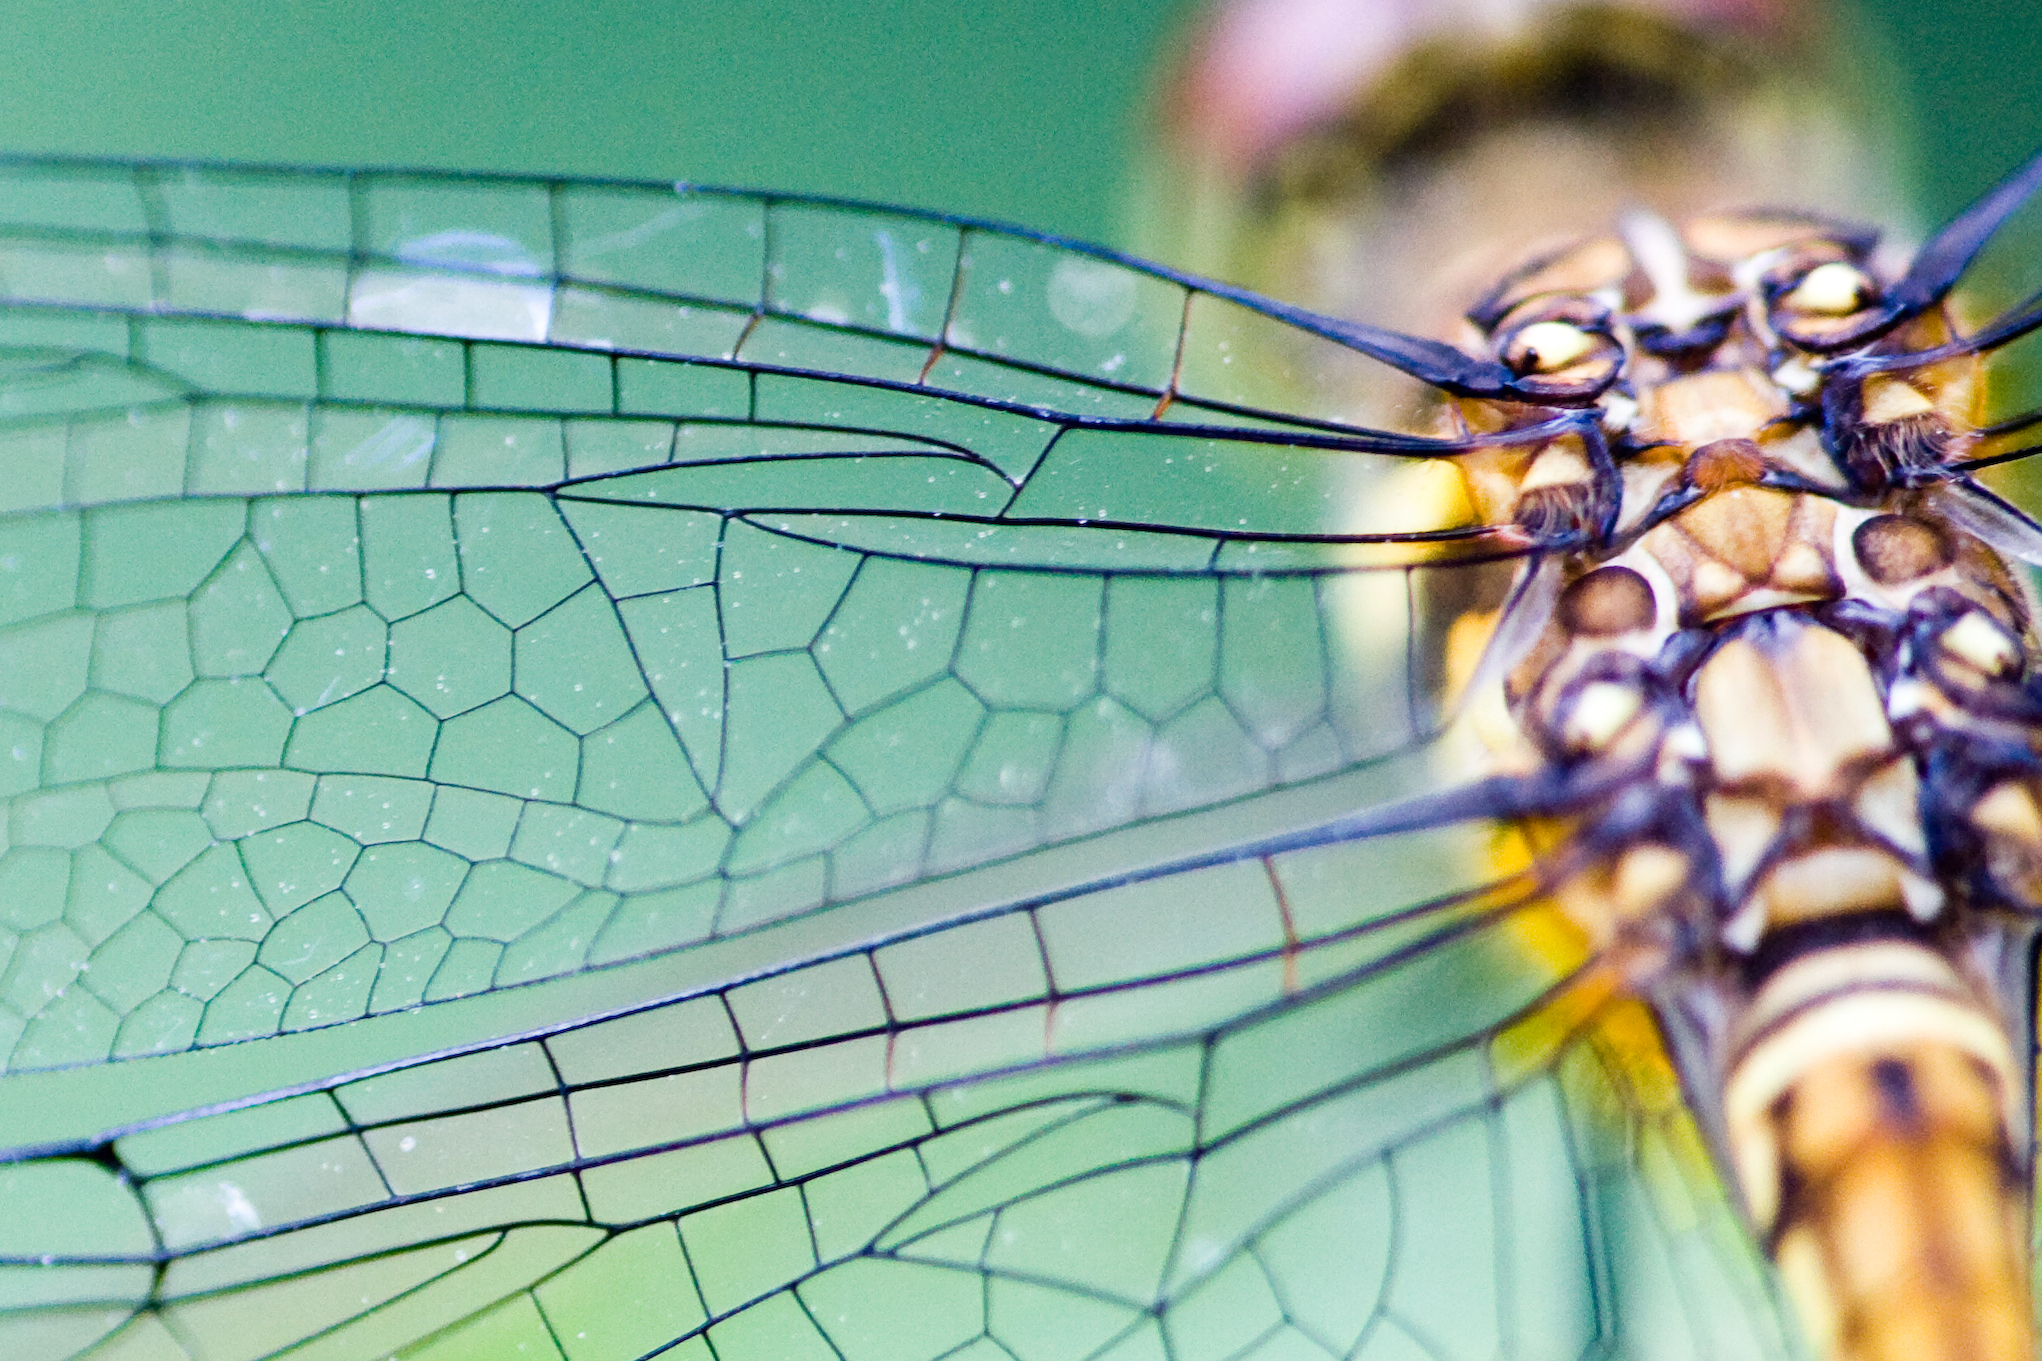
\includegraphics[width=0.7\linewidth]{pics/dragonfly_wing_joi_ito}
	\caption{The wings of a dragonfly. Credit: Joi Ito (CC BY 2.0)}
	\label{fig:dragonflywingjoiito}
\end{figure}


\section{Distributed Hash Tables}





\section{A Nontechnical Introduction to NP-Completeness}

\subsection{The Traveling Salesperson Problem (TSP)}
\subsection{The Longest Path Problem}
\subsection{The Rudrata/Hamiltonian Path Problem}
\chapter{Other Data Structures}
\section{Skip Lists}

\end{document}